\documentclass[a4paper,11pt]{article}
\usepackage[top = 1.5 in, bottom = 1 in, left = 1.5 in, right = 1.5 in]{geometry}
\usepackage[utf8]{inputenc}
\usepackage[T1]{fontenc}
\usepackage[british, finnish]{babel}
\usepackage{lmodern}
\usepackage{url}
\usepackage{color}
\usepackage{graphicx}
\usepackage{setspace}
\usepackage{biblatex}
\bibliography{lahteet}
\newcommand{\engl}[1]{\foreignlanguage{english}{\em #1}}
\hyphenation{jär-jes-tä-mis-al-go-rit-mi jär-jes-tä-mis-al-go-rit-me-ja jär-jes-tä-mis-al-go-rit-min}

\begin{document}
\title{Järjestämisalgoritmien suunnittelu grafiikkayksiköille}
\author{Laura Leppänen}
\date{\today}
\maketitle
\thispagestyle{empty}

\tableofcontents
\onehalfspacing

\newpage
\setcounter{page}{1}

\section{Johdanto}

Järjestäminen on yksi tunnetuimmista ja tutkituimmista laskennallisista ongelmista. Järjestämisalgoritmit ovat keskeisiä rakennuspalikoita esimerkiksi tietokantajärjestelmissä, hakumoottoreissa sekä tietokonegrafiikassa ja maantieteellistä dataa käsittelevissä järjestelmissä, joissa kohteita järjestetetään spatiaalisesti. Tästä johtuen tehokkaita järjestämisalgoritmeja tarvitaan kaikilla ohjelmointialustoilla, ja uusien arkkitehtuurien tarjoamia rinnakkaistamismahdollisuuksia on tarpeen käyttää hyödyksi.

Prosessorien ytimien määrä on jo pitkään ollut jatkuvassa kasvussa. Neliytimiset suorittimet ovat jo nykyään tavallisia, ja tulevaisuudessa kehitys näyttää menevän yhä vahvemmin ns. massiivimoniytimisten prosessorien (\engl{manycore processor}) suuntaan. Lisäksi ytimet kykenevät usein useamman säikeen suorittamiseen yhtäaikaisesti. Grafiikkayksiköissä massiivinen ytimien määrä on jo saavutettu: esimerkiksi nykyisissä Nvidian valmistamissa grafiikkayksiköissä ytimiä on jopa 448 kappaletta (Nvidia Tesla C2050/ C2070/C2075) \cite{nvidiafermi2010}.

Ytimien määrän lisäksi grafiikkayksiköiden ohjelmoinnissa täytyy ottaa huomioon, että ulkoiseen muistiin viittaaminen on hidasta, ja grafiikkapiirillä olevaa nopeaa muistia on rajallinen määrä \cite{leischner2010}. Täten muistissakäynnit on syytä suunnitella siten, että grafiikkayksikkö pystyy yhdistämään joukon muistiviittauksia yhdeksi viittaukseksi suurempaan muistialueeseen.

Esittelen seuraavassa luvussa lyhyesti CUDA-ohjelmointiympäristön ja ne grafiikkayksiköiden arkkitehtuuriset ominaisuudet, jotka algoritmien suunnittelussa on otettava huomioon. Sen jälkeen esittelen muutamia erityyppisiä järjestämisalgoritmeja ja niiden toteutuksia CUDA-ympäristössä.

\section{Rinnakkaislaskenta nykyisillä grafiikkayksiköillä}

\subsection{Tesla-näytönohjaimet ja CUDA-arkkitehtuuri}

Edellisen sukupolven Tesla-näytönohjaimissa (C1060) oli 30 moniprosessoria \\ (\engl{streaming multiprocessor}), joista jokainen koostuu kahdeksasta ytimestä (\engl{scalar processor}). Yhteensä fyysisiä ytimiä oli siis 240. Uusimman sukupolven Tes\-la-näy\-tön\-oh\-jai\-mis\-sa ytimiä on 448 jaettuna 14 moniprosessorille. Tesla-gra\-fiik\-ka\-yk\-si\-kön täydellinen hyödyntäminen kuitenkin edellyttää vähintään n. 5000\thinspace--\thinspace10\thinspace000 yhtäaikaisen säikeen käyttöä \cite{leischner2010}. Yksittäisellä Tesla C1060 -näytönohjaimen moniprosessorilla on mahdollista ajaa yhtäaikaisesti 1024 säiettä \cite{satish2009}.

Jokaisella moniprosessorilla on tietty näytönohjaimen sukupolvesta riippuva määrä rekisteritilaa. Lisäksi jokaisella moniprosessorilla on oma ydinten kesken jaettu muisti, jonka luku- ja kirjoitusoperaatiot ovat nopeita. Viittaukset ulkoiseen muistiin pyritään minimoimaan, koska ne ovat kalliita operaatioita. Myös kommunikointi moniprosessorien välillä on hidasta, joten algoritmit on syytä suunnitella siten, ettei synkronointia moniprosessorien välillä tarvita usein \cite{kolonias2011}.

Hallitakseen suurta määrää yhtäaikaisia säikeitä moniprosessorit käyttävät ns. SIMT-arkkitehtuuria (\engl{Single Instruction, Multiple Thread}) \cite{lindholm2008}. Moniprosessorin SIMT-käsky-yksikkö suorittaa säikeet 32 rinnakkaisen säikeen ryhmissä eli ns. loimissa (\engl{warp}, Lindholmin \cite{lindholm2008} mukaan termi on peräisin matonkudonnasta). Loimen säikeet ovat kaikki samaa tyyppiä, mutta käyttävät eri dataa.

CUDA-ohjelmointiympäristö (\engl{Compute Unified Device Architecture}) \cite{cudaprogramming} mahdollistaa rinnakkaisten ohjelmien ajamisen näytönohjaimilla. Tyypillisesti (sarjalliset) CUDA-isäntäsovellukset suoritetaan tavallisella suorittimella ja rinnakkaiset aliohjelmat (CUDA-ytimet, \engl{kernels}) näytönohjaimella.

CUDA-ytimet ovat sarjallisia sovelluksia, joita suoritetaan useassa säikeessä samanaikaisesti. Nämä säikeet järjestetään säielohkoiksi (\engl{thread block}) \cite{cudaprogramming}. Analysoitaessa CUDA-ohjelmointiympäristölle suunniteltuja algoritmeja voidaan ajatella käytettävien säielohkojen määrän vastaavan prosessorien määrää perinteisemmässä rinnakkaisalgoritmien analyysissa \cite{satish2009}.

\subsection{Suorituskyvyn tehostaminen}

Jotta näytönohjainten täyttä tehoa pystyttäisiin hyödyntämään, täytyy algoritmien suunnittelussa huomioida joitakin SIMT-arkkitehtuureihin liittyviä erityisominaisuuksia.

Loimeen kuuluvat säikeet suoritetaan siten, että jokainen säie suorittaa samaa käskyä samanaikaisesti, mutta kukin niistä käsittelee eri dataa (ns. SIMD-käskyt, \engl{Single Instruction, Multiple Data}). Jos kaksi säiettä haarautuu eri suuntiin valintalauseessa, valitut haarat suoritetaan peräkkäin --- ei siis rinnakkain \cite{leischner2010} \cite{cederman2009}. Tämä hidastaa suoritusta, joten täysi teho saavutetaan vain, jos kaikki saman loimen säikeet valitsevat saman suorituspolun. Eri loimien välisillä eroilla sen sijaan ei ole merkitystä suorituskyvyn kannalta \cite{leischner2010} \cite{satish2009}.

Suorituksen aikana data pidetään globaalissa muistissa, mutta siihen viittaaminen on melko hidasta. Kullakin moniprosessorilla on näytönohjainmallista riippuva määrä nopeaa paikallista muistia --- esimerkiksi Tesla C1060-näytönohjaimella 16 kilotavua moniprosessoria kohti. Laskennan aikana kannattaa siis käyttää paikallista jaettua muistia datan väliaikaiseen säilytykseen, koska viittauksia muistiin tulee paljon \cite{cederman2009} \cite{leischner2010}. Laskennan loputtua käsitelty data voidaan kopioida takaisin globaaliin muistiin.

Säikeet voivat periaatteessa viitata mihin tahansa kohtaan muistia, mutta muistiviittaukset kannattaa tehdä siten, että samaan loimeen kuuluvat säikeet viittaavat peräkkäisiin muistiosoitteisiin. Tällöin muistiviitteet voidaan muuntaa yhdeksi suureksi luku- tai kirjoitusoperaatioksi \cite{cederman2009} \cite{satish2009}. Paikallista jaettua muistia käytettäessä säikeiden kannattaa viitata eri muistipaikkoihin, koska muutoin luku- ja kirjoitusoperaatiot joudutaan taas suorittamaan sarjallisesti. Toisaalta jos kaikki säikeet viittaavat samaan muistipaikkaan, tulee muistiviitteestä taas yhtä nopea kuin yksittäisestä lukuoperaatiosta \cite{cederman2009}.

Kolonias ja kumppanit \cite{kolonias2011} huomauttavat lisäksi, että datan siirtäminen CPU:n ja CUDA-laitteiden välillä on usein niin hidasta, että mikäli osa laskennasta tehdään jo valmiiksi CPU:lla, voi järjestäminenkin olla tehokkaampaa suorittaa siellä ulkoisen CUDA-laitteen käyttämisen sijasta. Toisaalta CUDA Toolkitin versiosta 2.2 lähtien ohjelmoijan on mahdollista allokoida isäntäjärjestelmästä muistia, johon CUDA-ytimillä on suora pääsy \cite{kolonias2011}. Tällöin siirtäminen isäntäjärjestelmän ja näytönohjaimen välillä nopeutuu huomattavasti.

\section{Järjestämisalgoritmit CUDA-ympäristölle}

Tehokkaimpia tähän mennessä julkaistuja järjestämisalgoritmeja CUDA-ym\-pä\-ris\-töl\-le näyttävät kirjallisuuden perusteella olevan eri toteutukset lomitusjärjestämisestä (\engl{merge sort}) \cite{satish2009} \cite{satish2010}, kantalukujärjestämisestä (\engl{radix sort}) \cite{satish2009} \cite{merrill2011} ja laskentajärjestämisestä (\engl{counting sort}) \cite{kolonias2011}. Esimerkiksi Nvidian CUDA SDK:n ja CUDA Data-Parallel Primitives -kirjaston (CUDPP) \cite{cudpp} kantalukujärjestämisalgoritmit perustuvat Satishin ja kumppanien esitykseen \cite{satish2009}.

Myös järjestämisverkkoihin perustuvat algoritmit kuten Petersin ja Schulz-Hildebrandtin \cite{peters2012gems} esittelemä toteutus bitoniselle järjestämisalgoritmille (\engl{bitonic sort}) näyttävät lupaavalta lähestymistavalta massiivimoniytimisillä prosessoreilla suoritettavaan järjestämiseen. Lisäksi pikajärjestämisestä (\engl{quicksort}), jota on perinteisesti pidetty yhtenä nopeimmista lajittelualgoritmeista yksiytimisillä prosessoreilla, on tehty joitakin toteutuksia CUDAlle (mm. \cite{cederman2009}).

Lähestymistapa järjestämisalgoritmien suunnitteluun massiivimoniytimisillä prosessoreilla poikkeaa tavallisista moniydinprosessoreista siinä, että moniydinprosessoreilla tyypillisesti keskitytään eri toimintojen suorittamiseen rinnakkain, kun taas massiivimoniydinprosessoreilla suoritetaan samoja toimintoja rinnakkain eri datalle \cite{satish2009}.

\subsection{Kantalukujärjestäminen}

Kantalukujärjestäminen on kokonaislukuavainten järjestämiseen tarkoitettu algoritmi, joka perustuu luvun numeroiden järjestämiseen yksitellen vähiten merkitsevästä numerosta\footnote{Huom: Jos siis kantaluku (\engl{radix}) on 10, tarkoitetaan tässä numerolla kokonaislukuja 0\thinspace--\thinspace9. Kantaluku voisi kuitenkin olla esimerkiksi 2, jolloin käsiteltäisiin kokonaislukujen sijaan avaimen bittiesityksen yksittäisiä bittejä.} alkaen. Kun kokonaislukuavainten pituus on vakio $d$ ja avaimia on $n$ kappaletta, algoritmin aikavaativuus on $O(n)$.

Algoritmi käy avaimet läpi $d$ kertaa. Jokaisella läpikäynnillä avainjoukko järjestetään yksittäisen avaimen numeron perusteella käyttäen jotakin vakaata\footnote{Järjestämisalgoritmi on \emph{vakaa}, jos se säilyttää sellaisten arvojen alkuperäisen järjestyksen, joiden avaimet ovat yhtä suuret. Esimerkiksi parijono $(3, 7)$, $(3, 1)$ voidaan järjestää parin ensimmäisen alkion perusteella kahdella eri tavalla. Vakaan järjestämisalgoritmin tulos olisi $(3, 7)$, $(3, 1)$. Epävakaa järjestämisalgoritmi voisi tuottaa tuloksen $(3, 1)$, $(3, 7)$.} järjestämisalgoritmia, esimerkiksi laskentajärjestämistä \cite{clrs}. Juuri laskentajärjestämisen käyttäminen primitiivinä tekee kantalukujärjestämisestä helposti rinnakkaistuvan, sillä laskentajärjestäminen voidaan esimerkiksi helposti redusoida rinnakkaiseksi prefiksisummaoperaatioksi\footnote{Lukujonon $x_0, x_1, x_2, ..., x_n$ prefiksisumma on lukujono $x_0, x_0 + x_1, x_0 + x_1 + x_2, ..., x_0 + ... + x_n$.} \cite{satish2009}.

Satishin ja kumppanien \cite{satish2009} lähestymistavassa kantaluku on $2^b$, missä $b$ valitaan kokeellisesti. Tällöin kokonaislukuavaimen numerot ovat $b$ bitin jonoja. Tarvittavien muistiviitteiden (\engl{scatter}-operaatioiden) määrä pyritään minimoimaan valitsemalla $b > 1$. Data jaetaan 256 säikeen säielohkoihin, joista kukin käsittelee 1024 alkiota --- siis 4 alkiota säiettä kohti. Säielohkoja luodaan siis $p = \lceil n/1024 \rceil$ kappaletta \cite{satish2009}.

Jokaista kokonaislukuavaimen $k$ numeroa kohti lasketaan, monessako avaimessa esiintyy samassa kohtaa pienempi numero, ja kuinka monta sellaista avainta, joissa numero on sama, esiintyy aikaisemmin lukujonossa. Näiden kahden lukumäärän summa on avaimen $k$ indeksi eli aste (\engl{rank}) järjestämisen tuloksena saatavassa taulukossa \cite{satish2009}. Tehokkuuden vuoksi tämä tehdään siten, että jokainen säielohko laskee histogrammin sille annetun lukujoukon lukujen esiintymistä, jolloin asteet voidaan helposti laskea prefiksisumman avulla.

Läpikäynnit suoritetaan neljässä vaiheessa:
\begin{singlespace*}
\begin{enumerate}
\item Kukin säielohko järjestää sille kuuluvat alkiot paikallisessa nopeassa muistissa. Bitit käsitellään yksitellen siten, että iteraatioita tulee $b$ kappaletta.
\item Kukin säielohko kirjoittaa numeroiden esiintymähistogrammin ja järjestetyn datan globaaliin muistiin.
\item Lasketaan sarakkeittaisessa järjestyksessä (\engl{column-major order}) prefiksisumma $p$ kappaleesta histogrammitaulukoita. Ks. kuva \ref{fig:columnscan}.
\item Kukin säielohko kopioi alkionsa prefiksisummalla lasketun indeksin osoittamaan muistiosoitteeseen.
\end{enumerate}
\end{singlespace*}

\begin{figure}
\centering
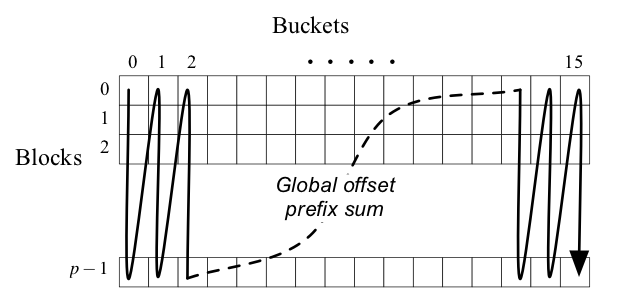
\includegraphics[scale = 0.5]{prefixsum}
\caption{Prefiksisumma sarakkeittaisessa järjestyksessä (kuvan lähde \cite{satish2009}). Taulukon rivit ovat eri säielohkojen tuottamia histogrammitaulukoita.}
\label{fig:columnscan}
\end{figure}

Kantaluvussa esiintyvän vakion $b$ valintaan vaikuttaa kaksi tekijää \cite{satish2009}. Toisaalta suuremmat $b$:n arvot heikentävät kohdassa (4) tapahtuvien \engl{scatter}-o\-pe\-raa\-ti\-oi\-den yhtenäisyyttä, koska mahdollisten numeroiden joukko on suurempi. Toisaalta jos $b$:n arvo on pienempi, joudutaan läpikäyntejä tekemään enemmän, jolloin jokaisen läpikäynnin lopussa suoritetaan uusi \engl{scatter}-operaatio muistiin. Molemmat ovat hidastavia tekijöitä. Kantaluvuksi $2^b$ valitaan empiirisen optimoinnin tuloksena $2^b = 16 = \sqrt{t}$, missä $b = 4$ ja $t = 256$ on säikeiden määrä yhdessä säielohkossa.

Kantalukujärjestämisen nopeus riippuu vahvasti avainten pituudesta, koska avainten ollessa lyhyempiä tarvitaan läpikäyntejä vähemmän (ks. kuva \ref{fig:radix_sort_varying_key_size}). Algoritmi kykenee järjestämään 8-bittisiä avaimia jopa yli 500 miljoonaa paria sekunnissa. 32-bittisten avaimien lajittelunopeus taas on korkeimmillaan lähellä 150 miljoonaa. Datan esijärjestämisellä ei ole oleellista merkitystä algoritmin nopeuden kannalta \cite{satish2009}.

\begin{figure}
\centering
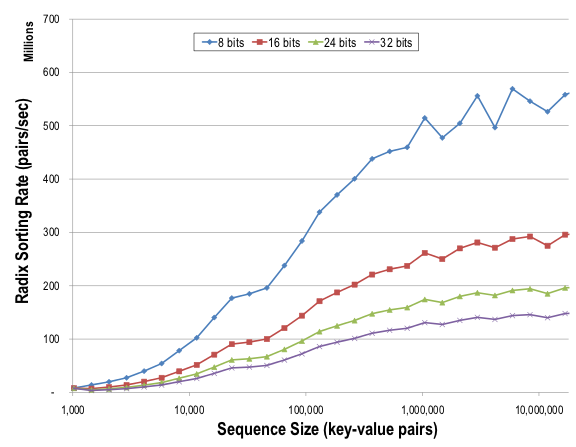
\includegraphics[scale = 0.45]{radix_sort_varying_key_size}
\caption{Kantalukujärjestämisen järjestämien parien määrä sekunnissa eri pituisilla avaimilla Nvidian GeForce GTX 280 -näytönohjaimella (kuvan lähde \cite{satish2009}).}
\label{fig:radix_sort_varying_key_size}
\end{figure}

Merrillin ja Grimshawn \cite{merrill2010} \cite{merrill2011} hiukan tuoreempi ja optimoidumpi kantalukujärjestämistoteutus suoriutuu lajittelusta huomattavasti nopeammin pitemmilläkin avaimilla. Nvidian GT200-sarjan näytönohjaimilla algoritmin sanotaan kykenevän lajittelemaan 482 miljoonaa 32-bittistä avain-arvo-paria tai 500 miljoonaa 32-bittistä avainta sekunnissa \cite{merrill2010}. Yleisesti toteutus on näytönohjaimesta riippuen noin kahdesta kolmeen kertaa CUDPP:n Satishin ja kumppanien esittelemään malliin pohjautuvaa algoritmia nopeampi \cite{merrill2011}. Tämä toteutus on todennäköisesti nopein tähän mennessä esitellyistä GPU-lajittelualgoritmeista.

\subsection{Lomitusjärjestäminen}

Satish ja kumppanit \cite{satish2009} ovat esitelleet myös yhden tehokkaimmista lomitusjärjestämisen toteutuksista CUDA-ympäristölle. Algoritmi suoritetaan kolmessa vaiheessa:

\begin{singlespace*}
\begin{enumerate}
\item Syötetaulukko jaetaan $p = \lceil n/1024 \rceil$ osaan kuten kantalukujärjestämisessä.
\item Osiot järjestetään $p$ kappaleessa rinnakkaisia säielohkoja.
\item Järjestetyt lohkot lomitetaan rinnakkaistetusti käyttäen parittaista $\log(p)$-syvyistä lomituspuuta.
\end{enumerate}
\end{singlespace*}

Vaiheessa (2) järjestämiseen käytetään Batcherin järjestämisverkkoihin perustuvaa \engl{odd-even merge sort} -algoritmia, joka on tehokas näytönohjaimilla \cite{kipfer2005gpugems}\footnote{Satishin \cite{satish2009} mukaan käytännön kokeissa 5-10\% tehokkaampi kuin suositumpi, myös järjestämisverkkoihin perustuva bitoninen lajittelu}. Algoritmin ajatus on, että parilliset ja parittomat avaimet järjestetään erillisinä joukkoina ja lopuksi lomitetaan. Satishin ja kumppanien lähestymistavassa parilliset ja parittomat avaimet lajitellaan eri säielohkoissa.

Valtaosa työstä tehdään lomitusvaiheessa. Jokaisella lomituspuun tasolla lomitetaan vaiheen (2) tuottamat järjestetyt lohkot parittomia ja parillisia avaimia keskenään pareittain. Koska lomitettavien parien määrä pienenee geometrisesti jokaisella lomituspuun tasolla, täytyy lomitusalgoritmia tehostaa. Satish ja kumppanit tekevät tämän käyttämällä hajota ja hallitse -tekniikkaa myös lomituspuun eri tasoilla, jolloin rinnakkaisuutta pystytään hyödyntämään myös parien vähentyessä. Lisäksi alkioiden lopullisten sijaintien laskenta tehdään käyttäen rinnakkaisia binäärihakuja \cite{satish2009}.

Jos lomitettavat (järjestetyt) lohkot ovat riittävän pieniä, korkeintaan $t = 256$ alkion kokoisia, voidaan lomitus tehdä yhdellä $t$ säikeen säielohkolla. Lomitettaessa järjestettyjä lohkoja $A$ ja $B$ järjestetyksi lohkoksi $C$ tarvitsee kullekin alkiolle $a_i \in A$ laskea $\mathrm{rank}(a_i, C)$, joka on alkion $a_i$ sijainti lohkossa $C$. Koska $A$ ja $B$ ovat järjestettyjä, tiedetään että $\mathrm{rank}(a_i, C) = i + \mathrm{rank}(a_i, B)$, missä $\mathrm{rank}(a_i, B)$ on niiden alkioiden $b_j \in B$ määrä, jotka ovat pienempiä kuin $a_i$. Vastaavasti voidaan laskea kaikkien $B$:n alkioiden sijainnit lomitetussa taulukossa.

Edellä kuvattu laskenta voidaan toteuttaa binäärihaulla. Tällöin jokainen säielohkon säie voi laskea sen vastuulla olevien alkioiden sijainnit lomitetussa taulukossa ja kirjoittaa alkiot oikeille paikoilleen muistissa \cite{satish2009}.

Jos lomitettavien taulukoiden koko on suurempi kuin $t$, ne jaetaan korkeintaan $t$ alkion lohkoihin, jotka voidaan lomittaa rinnakkain edellä kuvatulla tavalla. Jakaminen toteutetaan seuraavalla tavalla:

\begin{singlespace*}
\begin{enumerate}
\item Taulukoille $A$ ja $B$ rakennetaan jakajataulukot $S_A$ ja $S_B$ valitsemalla molemmista taulukoista $t$. alkio. Siis esimerkiksi $S_A = [a_t, a_{2t}, a_{3t}, ...]$.
\item Jakajataulukot $S_A$ ja $S_B$ lomitetaan taulukoksi $S = \mathrm{merge}(S_A, S_B)$.
\item $A$ ja $B$ jaetaan molemmat korkeintaan $t$ alkion pituisiksi taulukoiksi jakajataulukon $S$ avulla. Tämä toteutetaan laskemalla jokaiselle jakaja-alkiolle $s \in S$ $\mathrm{rank}(s, A)$ ja $\mathrm{rank}(s, B)$. Tämän jälkeen jakaja-alkioiden rajaamat osiot taulukoista $A$ ja $B$ voidaan lomittaa pareittain edellä kuvatulla tavalla käyttäen yhtä säielohkoa paria kohti.
\end{enumerate}
\end{singlespace*}

Toisin kuin kantalukujärjestämisessä, lomitusjärjestämisen nopeus ei muutu ratkaisevasti avainten koon mukaan (kuva \ref{fig:merge_sort_varying_key_size}). Toisaalta algoritmi on kertaluokkaa kantalukujärjestämista hitaampi. Parhaimmillaan algoritmi luokittelee noin 60 miljoonaa avain-arvo-paria sekunnissa. Vertailuihin perustuvana järjestämisalgoritmina lomitusjärjestäminen on kuitenkin kantalukujärjestämistä yleiskäyttöisempi \cite{clrs}.

\begin{figure}
\centering
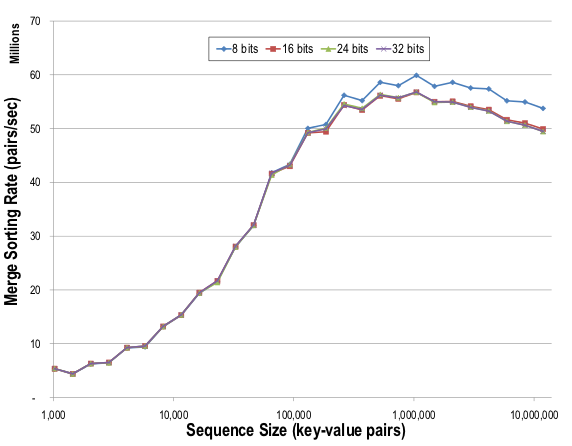
\includegraphics[scale = 0.45]{satish_mergesort}
\caption{Lomitusjärjestämisen järjestämien parien määrä sekunnissa eri pituisilla avaimilla Nvidian GeForce GTX 280 -näytönohjaimella (kuvan lähde \cite{satish2009}).}
\label{fig:merge_sort_varying_key_size}
\end{figure}

\subsection{Järjestämisverkot ja bitoninen järjestäminen}

Bitoninen järjestäminen (\engl{bitonic sort}) on Kevin Batcherin vuonna 1967 kehittämä järjestämisalgoritmi, joka perustuu järjestämisverkkoihin. Järjestämisverkko on abstrakti matemaattinen malli, joka muodostuu syötelangoista ja niitä yhdistävistä vertailumoduuleista. Järjestettävät syötteet ''liikkuvat'' syötelankoja pitkin vasemmalta oikealle. Kun syöteluvut pääsevät vertailumoduulin kohdalle, se vertaa lukuja toisiinsa ja tarvittaessa vaihtaa niiden paikkoja. Järjestämisverkon tekemien vertailuoperaatioiden määrä riippuu ainoastaan syötteen pituudesta, ei sisällöstä.

%\begin{figure}
%\centering
%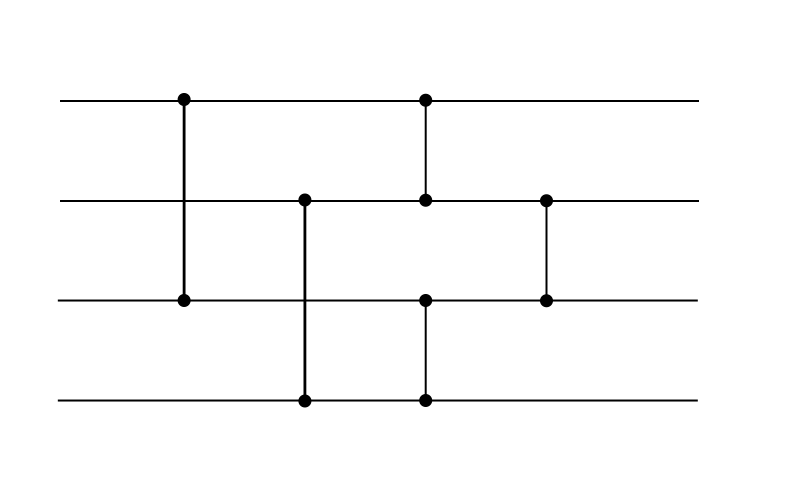
\includegraphics[scale = 0.45]{sortingnetwork}
%\caption{Yksinkertainen järjestämisverkko, joka koostuu neljästä syötelangasta ja viidestä vertailijasta.}
%\label{fig:sortingnetwork}
%\end{figure}

% Tähän bitonic sortin kuvaus.

Kuvassa \ref{fig:bitonicsort} on bitoninen järjestämisverkko kahdeksan alkion pituisille syötteille. Kuvassa numeroidut vaakaviivat ovat syötelankoja ja nuolet suunnattuja vertailu- ja vaihto-operaatioita. Vertailukohdissa nuolten molemmissa päissä olevia alkioita verrataan keskenään ja alkioista suurempi siirretään nuolenpään osoittamalle langalle.

Yleisesti $n = 2^k$ alkion pituisen syötteen bitoninen järjestämisverkko koostuu $k$ kappaleesta vaiheita $1,...,k$. Jokainen vaihe $p \in 1,...,k$ puolestaan koostuu $p$ kappaleesta askeleita $p, p-1, ..., 1$. Yhteensä bitonisessa järjestämisverkossa on siis $\sum_{i = 1}^k i = \frac{k \cdot (k + 1)}{2}$ askelta, joista kussakin suoritetaan $\frac{n}{2}$ vertailu- ja vaihto-o\-pe\-raa\-ti\-o\-ta.

\begin{figure}
\centering
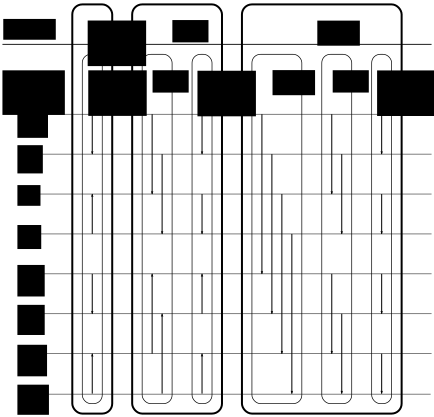
\includegraphics[scale = 0.8]{bitonic}
\caption{Bitoninen järjestämisverkko kahdeksalle alkiolle.}
\label{fig:bitonicsort}
\end{figure}

Kiinnostus järjestämisverkkoihin perustuvia algoritmeja kohtaan on kasvanut viime aikoina, koska ne on erityisesti suunnattu rinnakkaisia arkkitehtuureja varten. Rinnakkaistamisessa täytyy ottaa huomioon, että kun jokin vertailuoperaatio askeleessa $s$ alkaa käsitellä jotakin alkioparia, täytyy molempiin alkioihin kohdistuvien vertailuoperaatioiden olla suoritettu loppuun edellisessä askeleessa $s - 1$. Tämän vuoksi rinnakkainen toteutus vaatii tyypillisesti paljon rinnakkaisten prosessointiyksiköiden välistä synkronointia ja kommunikointia.

Peters ja Schulz-Hildebrandt \cite{peters2012gems} esittelevät GPU Computing Gems -kirjassa CUDA-toteutuksen bitoniselle järjestämiselle. Koska mielivaltaisten säikeiden synkronointi ei ole mahdollista CUDAssa, toiminnot pyritään suorittamaan oikeassa järjestyksessä siten, että synkronointia vaativat toiminnot sijoitetaan eri CUDA-ytimiin, jotka suoritetaan peräkkäin. Kommunikaatio peräkkäin suoritettavien CUDA-ytimien välillä toteutetaan käyttämällä näytönohjaimen globaalia muistia tiedonvälitykseen. Petersin ja Schulz-Hildebrandtin toteutus pyrkii minimoimaan kommunikaation ja synkronoinnin tarpeen tarvittavien CUDA-ytimien ja globaaliin muistiin tehtävien viitteiden vähentämiseksi.

Naiivi ratkaisu bitonisen järjestämisen rinnakkaistamiseen on luoda uusi säie jokaista yksittäistä vertailuoperaatiota varten (ks. kuva \ref{fig:bitonic_divided}, vasemmalla). Tällöin vertailuoperaatioiden suorittaminen oikeassa järjestyksessä varmistetaan suorittamalla verkko yksi askel kerrallaan siten, että edellinen askel on aina kokonaan suoritettu ennen seuraavan alkamista. Jokainen askel suoritetaan omana CUDA-ytimenään ja jokaisen askeleen jälkeen muuttunut syöte kirjoitetaan globaaliin muistiin, josta seuraava CUDA-ydin voi sen lukea. Tällöin CUDA-ytimiä tarvitaan yhtä monta kuin askeliakin, eli $n = 2^k$ alkion syötteelle $\frac{k \cdot (k + 1)}{2}$ kappaletta, joista jokainen koostuu $\frac{2^k}{2} = 2^{k-1}$ säikeestä, joista jokainen hakee käyttämänsä alkiot globaalista muistista, käsittelee yhden vertailu- ja vaihto-operaation ja kirjoittaa alkiot takaisin muistiin.

\begin{figure}
\centering
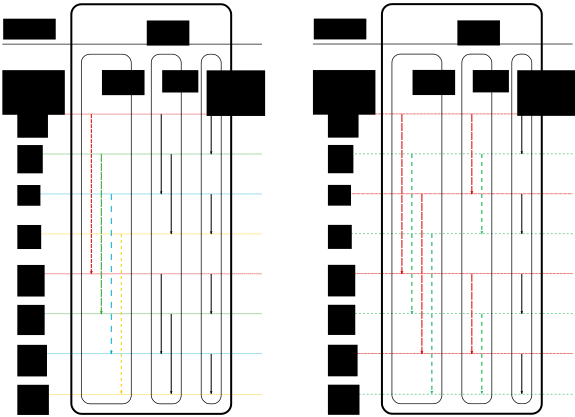
\includegraphics[scale = 0.8]{bitonic_divided}
\caption{Naiivi ratkaisu vasemmalla ja edistyneempi ratkaisu oikealla. Yksittäinen säie suorittaa samalla värillä merkityt vertailu- ja vaihto-operaatiot.}
\label{fig:bitonic_divided}
\end{figure}

Naiivin ratkaisun keskeisin ongelma on globaaliin muistiin tehtävien viittausten suuri määrä, joka hidastaa algoritmin suoritusta. Koska jokainen askel suoritetaan erikseen, tarvitaan jokaisessa CUDA-ytimessä $n$ luku- ja kirjoitusoperaatiota globaaliin muistiin. Lisäksi viittaukset globaaliin muistiin ovat paikoin epäyhtenäisiä \cite{peters2012gems}.

Peters ja Schulz-Hildebrandt \cite{peters2012gems} pyrkivät vähentämään tarvittavien muistiviitteiden määrää käyttämällä yhtä säiettä prosessoimaan vertailuoperaatioita useammasta peräkkäisestä askeleesta. Algoritmin oikeellisuuden varmistamiseksi pyritään löytämään sellaisia peräkkäisten askelten vertailuoperaatioita, jotka käsittelevät samaa joukkoa alkioita.

Edistyneempi ratkaisu on kuvattu kuvassa \ref{fig:bitonic_divided} oikealla. Kolmannen vaiheen askeleiden 3 ja 2 vertailu- ja vaihto-operaatiot on jaettu kahteen joukkoon. Samaan joukkoon kuuluvat vertailu- ja vaihto-operaatiot kohdistuvat tiettyyn neljän alkion joukkoon, johon ei kohdistu muita operaatioita. Tällöin askeleiden 3 ja 2 välillä ei tarvita lainkaan synkronointia ja käsiteltävät alkiot voidaan pitää säikeiden paikallisissa rekistereissä.

Pitempiä syötteitä käsiteltäessä voidaan ketjuttaa useampiakin askelia saman säikeen suoritettaviksi. Saman säikeen käsiteltäviksi annettavien askelten määrää rajoittaa kuitenkin säikeiden paikallisten rekisterien rajallinen määrä ja se, että näytönohjaimen tehokas hyödyntäminen edellyttää suurta määrää samanaikaisesti ajettavia säikeitä, joten säikeiden määrän ei haluta pienenevän merkittävästi \cite{peters2012gems}.

Rekisterien rajallisuus ei olisi ongelma, jos yksittäisten säikeiden sijaan käytettäisiin säielohkoja, jolloin säikeet voisivat käyttää paikallista jaettua muistia, joka on huomattavasti suurempi kuin säikeiden paikallinen rekisteritila. Tällöin kuitenkin ongelmaksi nousee se, että saman säielohkon käsiteltäviksi tulevat alkiot sijaitsevat harvoin peräkkäin muistissa, joten muistiin tehtävien viitteiden yhdistäminen ei ole mahdollista, mikä taas hidastaa suoritusta.

Jaettua muistia ja säielohkoja kuitenkin pystytään käyttämään hyödyksi toisella tavalla. Kun syötteenä saatavan avainjonon koko on $2^k$, kunkin vaiheen askeleissa $s, s-1, ..., 1$ käsitellään itsenäisesti $2^{k-s}$ kappaletta $2^s$ alkion alijonoja, jotka sijaitsevat peräkkäin muistissa. Jos tällainen $2^s$ alkion alijono mahtuu kokonaan säielohkon jaettuun muistiin, se voidaan siirtää globaalista muistista jaettuun muistiin yhdellä yhdistetyllä lukuoperaatiolla ja jakaa säielohkon sisällä vertailuoperaatiot säikeiden kesken edellä kuvatulla tavalla, mutta käyttäen rekisterien sijaan säielohkon jaettua paikallista muistia ja useiden CUDA-ytimien käynnistämisen sijaan lohkojen sisäistä synkronointia.

\section{Yhteenveto}

...

\printbibliography

\end{document}
